\documentclass{article}

\PassOptionsToPackage{numbers, compress}{natbib}
\usepackage[preprint]{neurips_2026}

\usepackage[utf8]{inputenc}
\usepackage[T1]{fontenc}
\usepackage{hyperref}
\usepackage{url}
\usepackage{booktabs}
\usepackage{amsfonts}
\usepackage{amsmath}
\usepackage{microtype}
\usepackage{xcolor}
\usepackage{graphicx}
\usepackage{tikz}
\usetikzlibrary{positioning, arrows.meta}

\newcommand{\popqa}{PopQA}
\newcommand{\todo}[1]{\textcolor{red}{[#1]}}

\title{ConceptFormer-2: Token-Efficient Grounding of Frozen\\
  Instruction-Tuned Language Models in Knowledge Graphs}

\author{%
  Joel Barmettler\thanks{Draft — author list and contributions preliminary. All numbers trace
  to per-item evaluation dumps and W\&B run ids in the project repository
  (\texttt{joelbarmettlerUZH/ConceptFormer}, branch \texttt{conceptformer-v2}).} \\
  University of Zurich\\
  \texttt{joel.barmettler@uzh.ch}\\
  \And
  Abraham Bernstein\\
  University of Zurich\\
  \And
  Luca Rossetto\\
  affiliation TBD\\
}

\begin{document}

\maketitle

\begin{abstract}
  We present ConceptFormer-2, which grounds a \emph{frozen}, instruction-tuned language model
  in a knowledge graph by compressing an entity's 1-hop neighborhood into $k$ continuous
  \emph{concept tokens} spliced into the model's input embeddings --- replacing $\sim$100 tokens
  of retrieved text with $k\!\approx\!8$. The encoder, a small Perceiver-style resampler over
  the frozen model's own label embeddings, is inductive (unseen entities require one forward
  pass) and trains \emph{label-free} by full-vocabulary KL self-distillation against the same
  frozen model reading the facts as text. On the full 14{,}266-question \popqa{} benchmark,
  $k{=}8$ concept tokens lift a frozen Qwen3-0.6B from 0.103 to 0.477 exact-match on unseen
  entities --- $2.6$--$3.2\times$ better than question-aware retrieval or LLM-written summaries
  at the same token budget --- while an untrained-injection control stays near floor, showing
  the learned compression carries the effect. Accuracy rises monotonically in $k$ through
  $k{=}32$ on matched curves at two corpus scales, exposing a three-way trade between token
  budget, training data, and model size: unseen-entity accuracy grows $2.3\times$ when training
  entities grow $10\times$, and additional tokens partially substitute for additional data.
  Counterfactual edge-swap probes show the model genuinely \emph{reads} the injected graph,
  increasingly so with $k$, while off-topic behavior is preserved (median next-token KL
  $\le$0.08 nats). ConceptFormer-2 turns a frozen conversational model into an
  entity-grounded QA system at roughly one-tenth the context cost of retrieval, with all
  corpora, checkpoints, and per-item evaluation outputs released.
\end{abstract}

\section{Introduction}

Instruction-tuned language models answer questions about popular entities from their weights
and fail on the long tail --- a deficit that persists even in frontier models, which encode far
more long-tail facts than they can recall \citep{emptyshelves,headtotail}. The standard remedy,
retrieval-augmented generation \citep{rag}, restores factuality but pays for it on every query:
a single entity's verbalized Wikidata neighborhood occupies a median of $\sim$100 context
tokens in our corpora, competing with the user's actual task for context budget, latency, and
key--value cache.

ConceptFormer \citep{cfv1} proposed a third channel: compress the knowledge-graph neighborhood
itself into a few \emph{continuous} tokens that a frozen LM consumes natively. The original
system was validated on GPT-2 (0.1B) with rank-based metrics on next-token factual recall and
received the best paper award of its hosting workshop at The Web Conference 2026. It left the
harder questions open: does latent injection survive \emph{generative, exact-match QA with a
modern conversational model}? Does the model actually \emph{read} the injected structure, or
merely absorb a text-like signal? And --- decisive for whether the channel matters at scale ---
what governs its value: the token budget $k$, the amount of knowledge the encoder is trained
on, or the size of the frozen model?

ConceptFormer-2 answers these questions with a redesigned system and a measurement-first
methodology. Three design changes carry most of the weight: (i) an \emph{inductive} featurizer
that represents each graph edge with the frozen model's own label embeddings --- replacing v1's
per-entity lookup table, so unseen entities need labels, not pretrained vectors; (ii) a
\emph{label-free} training objective --- full-vocabulary KL distillation of the frozen model
reading $k$ concept tokens against the \emph{same} frozen model reading the facts as text ---
requiring no annotated QA anywhere; and (iii) a zero-initialized output projection that makes
the student bit-identical to the frozen model at step~0, preserving capability by construction.

\paragraph{Contributions.}
\textbf{(1)}~A modernized latent knowledge-injection system for frozen instruction-tuned LLMs,
evaluated with generative exact match on the full \popqa{} benchmark, with strong text
baselines (question-aware retrieval, LLM-written budgeted summaries) and an untrained-injection
control (\S\ref{sec:efficiency}).
\textbf{(2)}~Matched token-budget curves at two corpus scales showing monotone gains through
$k{=}32$ and a three-way trade structure: data scales injection up ($2.3\times$ for $10\times$
entities), tokens partially substitute for data, and we measure the frozen-model-size axis
across the Qwen3 family (\S\ref{sec:scaling}).
\textbf{(3)}~Causal evidence that the model reads the injected graph --- counterfactual
edge-swap following that scales from $\sim$1\% ($k{=}1$) to $\sim$34\% ($k{=}32$) --- alongside
capability preservation and prompt robustness (\S\ref{sec:probes}).
\textbf{(4)}~An open release: corpora with per-teacher distillation targets, all checkpoints,
the evaluation harness, and per-item outputs enabling third-party paired re-analysis.

\section{Related work}
\label{sec:related}

\paragraph{Lineage.} The problem framing descends from language-models-as-knowledge-bases
probing \citep{lama,roberts} and its long-tail refinement \citep{headtotail,emptyshelves}, with
RAG \citep{rag} as the deployed remedy. Knowledge-enhanced PLMs inject KG signal by modifying
the model --- KnowBERT \citep{knowbert}, K-BERT \citep{kbert}, K-Adapter \citep{kadapter} ---
which our frozen-model constraint rules out. ConceptFormer v1 \citep{cfv1} injected
\emph{pretrained} KG node embeddings (TransE-family vectors at PyTorch-BigGraph scale
\citep{transe,pbg}) through a per-entity lookup table; the present system replaces this with
features built from the frozen model's own label embeddings, which is what makes the encoder
inductive. Prepending \emph{learned continuous tokens} to a frozen model descends from
prefix-tuning and soft prompts \citep{prefixtuning,lester,qineisner}, textual inversion
\citep{textualinversion}, and most directly Frozen \citep{frozenlm} and Flamingo
\citep{flamingo}. Our substrate is Wikidata \citep{wikidata}; graph verbalization baselines
follow the graph-to-text encoding line \citep{talklikeagraph}.

\paragraph{Soft-token context compression.} Gist tokens \citep{gist} and AutoCompressor
\citep{autocompressor} adapt the LM itself; ICAE \citep{icae} and 500xCompressor
\citep{fivehundredx} train LoRA encoders against frozen decoders with reconstruction
objectives; CompLLM \citep{compllm} distills per-segment embeddings via activation matching;
ARC-Encoder \citep{arcencoder} is the strongest recent frozen-decoder text compressor. PISCO
\citep{pisco} shares our sequence-distillation family but reports that frozen decoders
underperform (their Appendix~G) --- a claim our frozen-decoder results contradict at entity
granularity. Closest is xRAG \citep{xrag}: frozen decoder, input-embedding injection,
same-model KL distillation --- but xRAG \emph{translates} a single pre-existing retriever
vector rather than learning compression, is retriever-bound at inference, and evaluates neither
unseen-entity generalization nor faithfulness. Cartridges \citep{cartridges} distills a KV
cache \emph{per corpus} by gradient descent: no amortization, no unseen items. None of these
compress \emph{structured} input, and none runs causal probes on the compressed representation
(post-hoc overflow probing \citep{overflow} being the nearest attempt).

\paragraph{Knowledge-graph injection into LLMs.} GNP \citep{gnp}, GraphToken \citep{graphtoken},
G-Retriever \citep{gretriever}, and LLaGA \citep{llaga} encode graphs into soft prompts
\emph{per question} with task cross-entropy on labeled QA; none precomputes reusable per-entity
tokens. KBLaM \citep{kblam} precomputes one key--value pair per \emph{triple}, injected into
every attention layer through modified attention, evaluated on synthetic KBs. Knowledge Prompts
\citep{knowledgeprompts} is the closest precompute precedent --- per-entity soft prompts for
1.1M Wikidata entities --- but as a lookup table of free parameters, making unseen entities
impossible by construction. Recent analyses find graph-token LLMs ``do not fully understand
graph tokens'' \citep{gteval} and that graph tokens can decouple from graph semantics
\citep{sink}; our counterfactual evaluation (\S\ref{sec:probes}) is designed to measure exactly
this. No prior work combines an amortized \emph{inductive} per-entity encoder, label-free
same-model distillation, unseen-entity and causal evaluation, and corpus scale.

\section{Method}
\label{sec:method}

\begin{figure}[t]
  \centering
  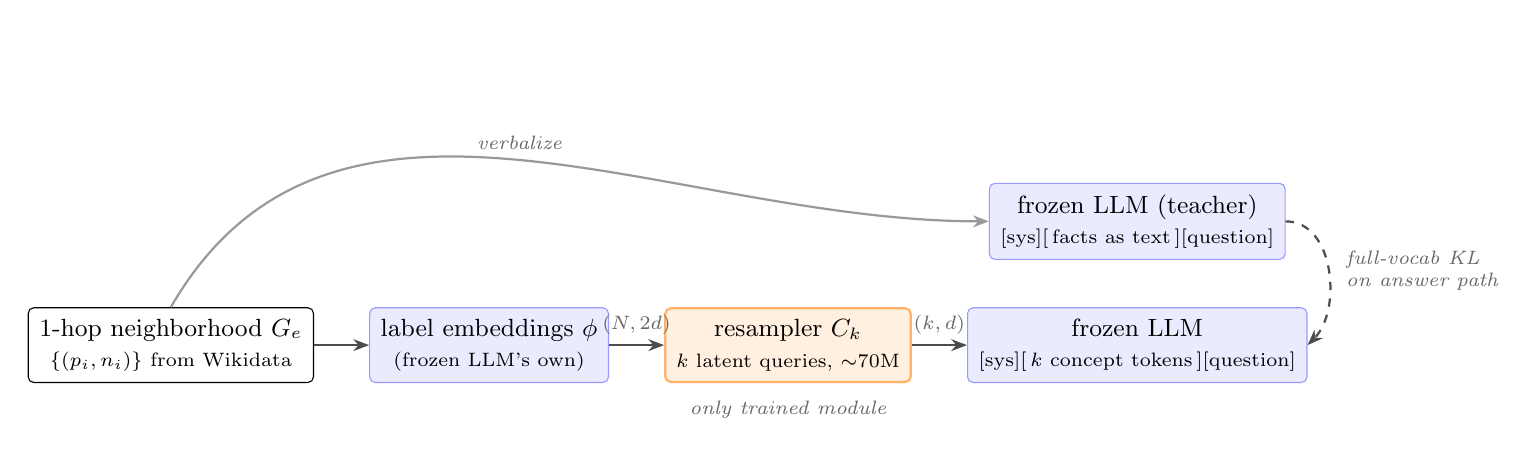
\begin{tikzpicture}[
    font=\small, node distance=4mm and 7mm,
    box/.style={draw, rounded corners=2pt, minimum height=7mm, inner sep=4pt, align=center},
    frozen/.style={box, fill=blue!8, draw=blue!40},
    train/.style={box, fill=orange!12, draw=orange!60, thick},
    lab/.style={font=\scriptsize\itshape, text=black!60},
    arr/.style={-{Stealth[length=2mm]}, thick, black!70}]
    \node[box] (kg) {1-hop neighborhood $G_e$\\ \scriptsize $\{(p_i, n_i)\}$ from Wikidata};
    \node[frozen, right=of kg] (feat) {label embeddings $\phi$\\ \scriptsize (frozen LLM's own)};
    \node[train, right=of feat] (enc) {resampler $C_k$\\ \scriptsize $k$ latent queries, $\sim$70M};
    \node[frozen, right=of enc, minimum width=34mm] (llm)
      {frozen LLM\\ \scriptsize $[\text{sys}][\,k \text{ concept tokens}\,][\text{question}]$};
    \node[frozen, above=6mm of llm, minimum width=34mm] (teacher)
      {frozen LLM (teacher)\\ \scriptsize $[\text{sys}][\,\text{facts as text}\,][\text{question}]$};
    \draw[arr] (kg) -- (feat);
    \draw[arr] (feat) -- node[above, lab]{$(N, 2d)$} (enc);
    \draw[arr] (enc) -- node[above, lab]{$(k, d)$} (llm);
    \draw[arr, dashed] (teacher.east) to[out=0, in=45]
      node[right=1mm, lab, align=left]{full-vocab KL\\ on answer path} (llm.east);
    \draw[arr, black!40] (kg.north) to[out=60, in=180]
      node[above, lab]{verbalize} (teacher.west);
    \node[lab, below=1mm of enc] {only trained module};
  \end{tikzpicture}
  \caption{ConceptFormer-2. Edge features are the frozen model's own mean-pooled label
  embeddings (inductive: any labeled entity works); a Perceiver-style resampler compresses the
  edge set into $k$ concept tokens spliced into the frozen model's input. Training minimizes
  the full-vocabulary KL between the same frozen model reading facts as text (teacher) and
  reading $k$ tokens (student), along the teacher's greedy answer path --- no QA labels, no
  LLM updates.}
  \label{fig:method}
\end{figure}

\paragraph{Setup and featurizer.} Let $M$ be a frozen chat LLM with input-embedding dimension
$d$. For an entity $e$ with 1-hop neighborhood $G_e = \{(p_i, n_i)\}_{i=1}^{N}$ (property and
neighbor labels, PageRank-ordered), each edge becomes
$x_i = [\,\phi(p_i);\phi(n_i)\,] \in \mathbb{R}^{2d}$, where $\phi$ mean-pools $M$'s input
embeddings over a label's tokens. Features are inductive and live in a space $M$ already
understands; no per-entity parameters exist anywhere.

\paragraph{Encoder.} A latent-query resampler \citep{perceiver,flamingo}: $k$ learned queries
cross-attend over the masked, permutation-invariant edge set, self-attend, and pass through a
feed-forward block, for $L$ layers ($d_{\text{model}}{=}1024$, $L{=}4$, $\sim$70M parameters
--- an encoder capacity ablation appears in Table~\ref{tab:ablations}); an output projection
maps to $\mathbb{R}^{k \times d}$. The projection is \emph{zero-initialized}, so at step~0 the
student is bit-identical to the frozen model; we found this variant more stable than a
multiplicative gate.

\paragraph{Objective.} The teacher is $M$ reading
$[\text{system}][\text{verbalized } G_e][\text{question}]$; its greedy answer path $y_{1..m}$ is
stored offline. The student is $M$ reading $[\text{system}][C_k(G_e)][\text{question}]$, with
the concept block occupying a contiguous unit-step RoPE span. The loss is the token-level
full-vocabulary forward KL along the stored path,
\begin{equation}
  \mathcal{L} = \frac{\tau^2}{m}\sum_{t=1}^{m}
  \mathrm{KL}\!\left( p_M(\cdot \mid \text{facts}, q, y_{<t}) \,\|\,
                      p_M(\cdot \mid C_k(G_e), q, y_{<t}) \right), \qquad \tau = 1.
\end{equation}
Only the $\sim$20 path positions pass through the LM head, keeping training memory-light; one
converged run fits a single 24\,GB consumer GPU. Corpus questions (generated by a separate LLM
from the graphs; below) exist solely to give the teacher something to answer --- no QA labels
enter the loss.

\paragraph{Data.} From the Wikidata PageRank ranking we sample entity pools
(\popqa{} subjects excluded), snapshot complete 1-hop neighborhoods, generate questions with an
open-weights Gemma model, \emph{tier} each question by whether the graph demonstrably helps the
backbone (base fails, facts-in-context succeeds; a 30\% sample of base-known questions is
retained), and store teacher paths. Corpora: 10k entities ($92{,}177$ rows under the
Qwen3-0.6B teacher) and 100k entities ($925{,}178$ rows). Tiering and teacher paths are
teacher-relative, so each backbone trains on its own corpus variant of near-identical size ---
comparisons across backbones are of ``each model with its own curriculum''.

\paragraph{Training.} AdamW, lr $10^{-4}$ held constant, weight decay $0.01$, effective batch
32 via gradient accumulation, 72k optimizer steps on the 10k corpus and 100k steps
($\approx$4 epochs) on the 100k corpus, best-checkpoint selection on a held-out sample. Every
reported configuration uses $\ge$3 random seeds.

\section{Evaluation protocol}
\label{sec:protocol}

All results are bracketed by two conditions of the same frozen model: \textbf{base} (no
knowledge; the floor) and \textbf{RAG} (facts as text with the questioned edge guaranteed
present; the ceiling, 0.96 on full \popqa{}). The metric is greedy exact match with word-boundary
alias matching; we additionally report the official (more lenient) \popqa{} metric, which
tracks ours within $\sim$0.5\,pt. Three accuracy axes: \textbf{held-out} (unseen questions
about trained entities), \textbf{held-in} (trained questions; an overfitting gauge), and
\textbf{\popqa{}} (unseen \emph{entities} --- the axis that requires inductive generalization
and is the paper's headline).

Four protocol properties matter for the statistics we report. (1)~\popqa{} is evaluated on the
\emph{full} benchmark ($n{=}14{,}266$ questions with snapshot coverage), bringing binomial
noise to $\sim$0.4\,pt. (2)~Held-out splits are \emph{fact-level}: paraphrases of the same
(entity, fact) never straddle train/test, and held-out sets are additionally filtered so no
tested fact was supervised. (3)~Evaluation subsets are frozen and shared across all runs,
configurations, and seeds, so any two systems can be compared item-by-item; we report Wilson
intervals and exact McNemar tests on shared items. (4)~Definitive numbers come from re-scoring
selected checkpoints on large, disjointly-sampled sets, never from the trajectory samples used
for checkpoint selection. Per-item outputs for every evaluation are released.

\section{Results}

\subsection{Token efficiency against strong text baselines}
\label{sec:efficiency}

\begin{figure}[t]
  \centering
  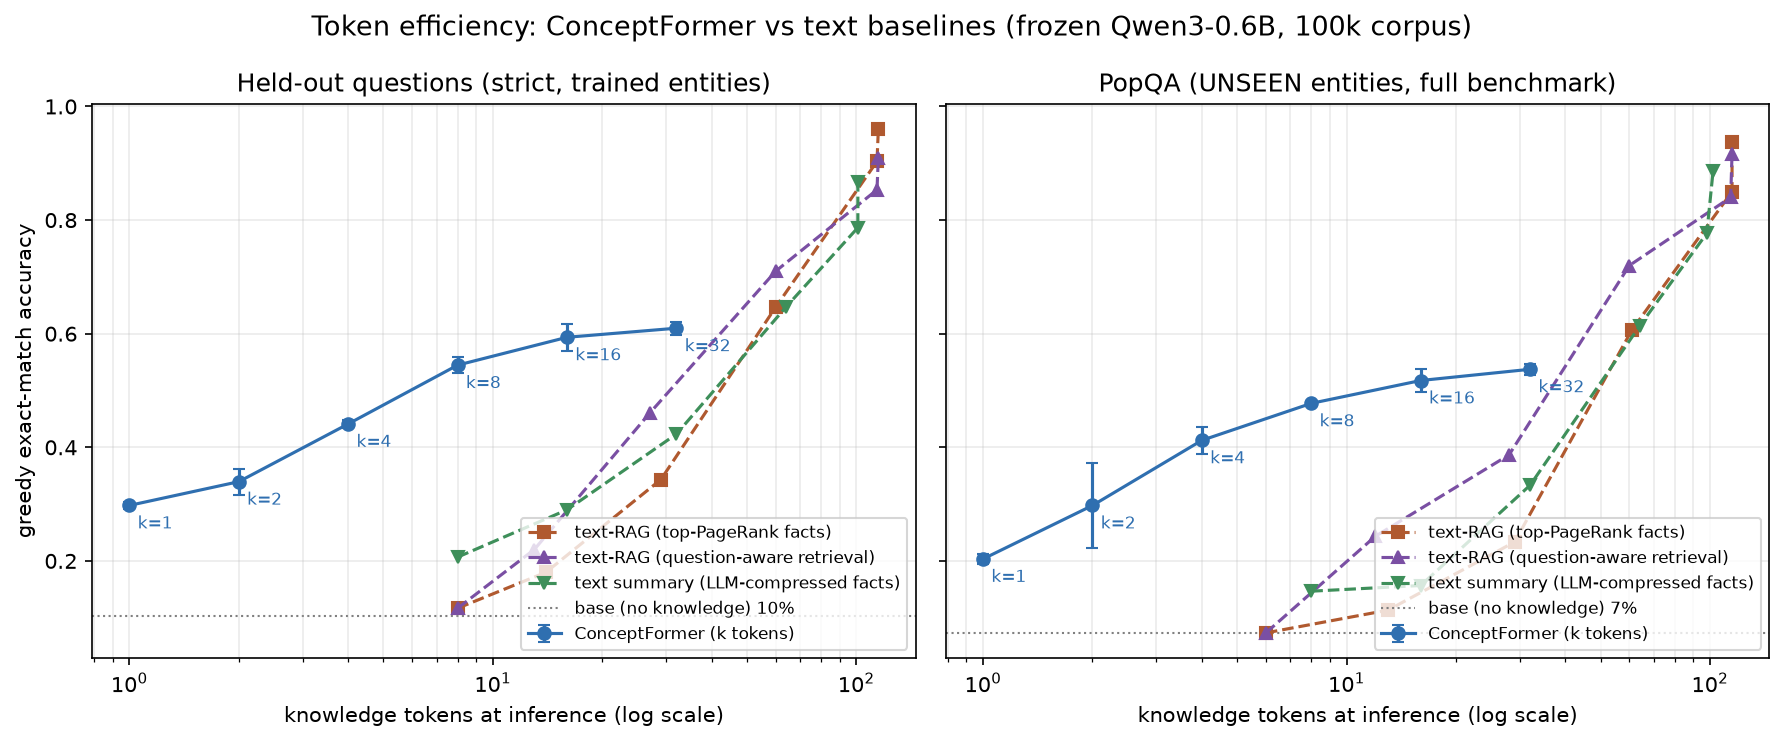
\includegraphics[width=\linewidth]{figures/token_efficiency.png}
  \caption{Accuracy vs.\ knowledge tokens spent at inference (log scale), frozen Qwen3-0.6B,
  100k-entity corpus, 3 seeds. Concept tokens dominate all three text baselines below
  $\sim$32 tokens on both axes; text catches up only at 64--128 tokens (most of a verbalized
  neighborhood). Left: strict held-out; right: full \popqa{}.}
  \label{fig:efficiency}
\end{figure}

Figure~\ref{fig:efficiency} compares concept tokens against three text baselines at matched
knowledge-token budgets: query-independent top-PageRank truncation, \emph{question-aware}
retrieval (facts ranked by embedding similarity to the question --- an advantage our
query-independent tokens do not have), and LLM-written budgeted summaries. At an 8-token budget
on unseen entities, concept tokens reach $0.477$ where the best text baseline reaches $0.147$;
at 16 tokens, $0.518$ vs.\ $0.243$. Text requires 64--128 tokens for parity, i.e., matched
accuracy costs text $\sim$5--6$\times$ more tokens. Two controls anchor the comparison. First,
filling the same $k$ slots with \emph{untrained} mean-pooled embeddings of the top-$k$ edges
scores $0.130$ on \popqa{} (base $0.103$), identically for $k{=}8$ and $16$: the learned
compression carries $\sim$93\% of the injected-knowledge effect. Second, the teacher/RAG
ceiling ($0.960$) confirms ample headroom remains.

\begin{table}[t]
  \caption{Corrected $k$-family on the 100k-entity corpus (frozen Qwen3-0.6B, 3 seeds,
  mean$\pm$std). Strict held-out $n{=}2000$; full \popqa{} $n{=}14{,}266$; official \popqa{}
  metric for literature comparability. Brackets: base $0.103$ (official $0.107$), RAG $0.960$.
  All adjacent $k$-contrasts are significant under item-paired McNemar (largest $p \approx
  10^{-6}$).}
  \label{tab:kfamily}
  \centering
  \small
  \begin{tabular}{lcccccc}
    \toprule
    $k$ & 1 & 2 & 4 & 8 & 16 & 32\\
    \midrule
    held-out & $.298{\pm}.006$ & $.340{\pm}.023$ & $.441{\pm}.007$ & $.545{\pm}.014$ & $.594{\pm}.024$ & $.610{\pm}.011$\\
    \popqa{} & $.203{\pm}.008$ & $.298{\pm}.075$ & $.412{\pm}.023$ & $.477{\pm}.002$ & $.518{\pm}.020$ & $.537{\pm}.010$\\
    \popqa{} (official) & $.207{\pm}.009$ & $.303{\pm}.077$ & $.419{\pm}.024$ & $.483{\pm}.002$ & $.523{\pm}.021$ & $.543{\pm}.010$\\
    \bottomrule
  \end{tabular}
\end{table}

\subsection{The three-way trade: tokens, data, and model size}
\label{sec:scaling}

\begin{figure}[t]
  \centering
  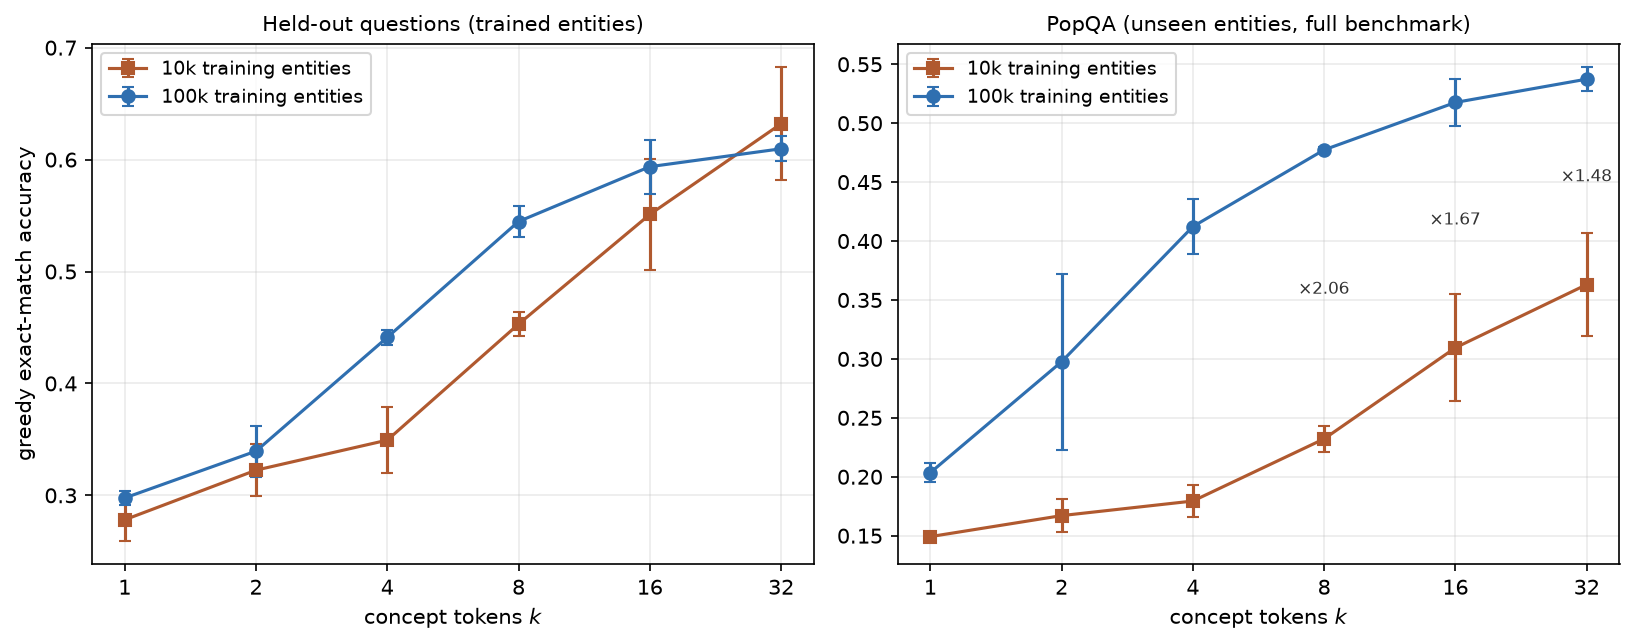
\includegraphics[width=\linewidth]{figures/fig_kcurves.png}
  \caption{Matched token-budget curves at two corpus scales (3 seeds, identical protocol).
  Accuracy rises monotonically in $k$ through $k{=}32$ at both scales. Annotations on the
  right panel give the 10k$\to$100k \popqa{} ratio per $k$: the data-scaling gain shrinks as
  $k$ grows --- additional tokens partially substitute for additional training data.}
  \label{fig:kcurves}
\end{figure}

\paragraph{Token axis.} Table~\ref{tab:kfamily} and Figure~\ref{fig:kcurves}: accuracy is
monotone in $k$ through $k{=}32$ on \emph{both} corpora, with every adjacent contrast
item-paired significant at 100k. Returns per token diminish --- $k{=}8$ buys $\sim$89\% of
$k{=}32$'s \popqa{} at a quarter of the tokens --- so the efficiency-optimal budget is a
deployment choice, not a capacity cliff.

\paragraph{Data axis.} Scaling training entities $10\times$ (identical eval sets, matched
placement, $k{=}8$) lifts full-\popqa{} accuracy from $0.210 \pm 0.012$ to $0.477 \pm 0.002$
--- a $2.3\times$ gain in unseen-entity generalization that had not saturated at the end of
training. Held-out rises too ($0.416 \to 0.545$) while held-\emph{in} falls
($\sim$0.82 $\to \sim$0.64): with more entities the encoder memorizes individual training
entities less and learns the edge$\to$concept mapping more --- the signature of
graph-learning rather than corpus memorization.

\paragraph{Token--data substitution.} The matched curves expose an interaction: the
10k$\to$100k \popqa{} ratio falls from $2.05\times$ ($k{=}8$) to $1.68\times$ ($k{=}16$) to
$1.48\times$ ($k{=}32$). A larger token budget extracts more value from a small training
corpus, partially substituting for data --- consistent with a rate--distortion view in which
both $k$ and corpus size bound how much neighborhood structure the encoder can faithfully
transmit.

\begin{figure}[t]
  \centering
  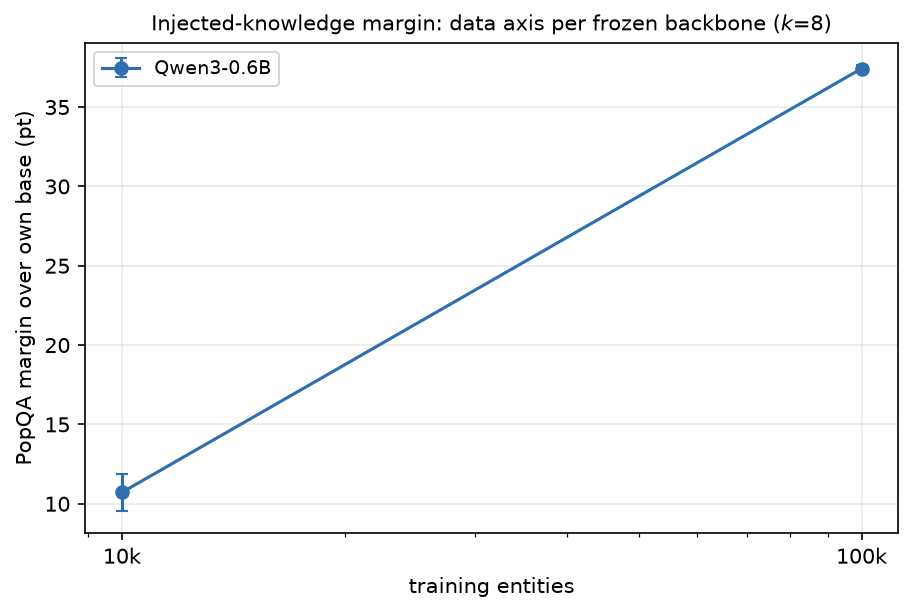
\includegraphics[width=0.62\linewidth]{figures/fig_grid.png}
  \caption{The data $\times$ model grid ($k{=}8$): \popqa{} margin over each frozen backbone's
  own base accuracy. \todo{1.7B and 4B cells land as training completes; figure regenerates
  from the same script.}}
  \label{fig:grid}
\end{figure}

\paragraph{Model axis.} We repeat the data transect across the Qwen3 family (0.6B, 1.7B, 4B),
each backbone with its own teacher-relative corpus and brackets (Figure~\ref{fig:grid}).
\todo{Pending cells: 1.7B $\times$ \{10k, 100k\} and 4B $\times$ \{10k, 100k\} at $k{=}8$
(and $k{=}16$ at 1.7B), 3 seeds each --- training in progress; this subsection's claims will
be finalized from those cells.} The question the grid answers: does a larger frozen model ---
which knows more of \popqa{} parametrically --- gain less from injection at fixed data, and if
so, does more data close the gap?

\subsection{Does it read the graph? Causal probes}
\label{sec:probes}

\begin{figure}[t]
  \centering
  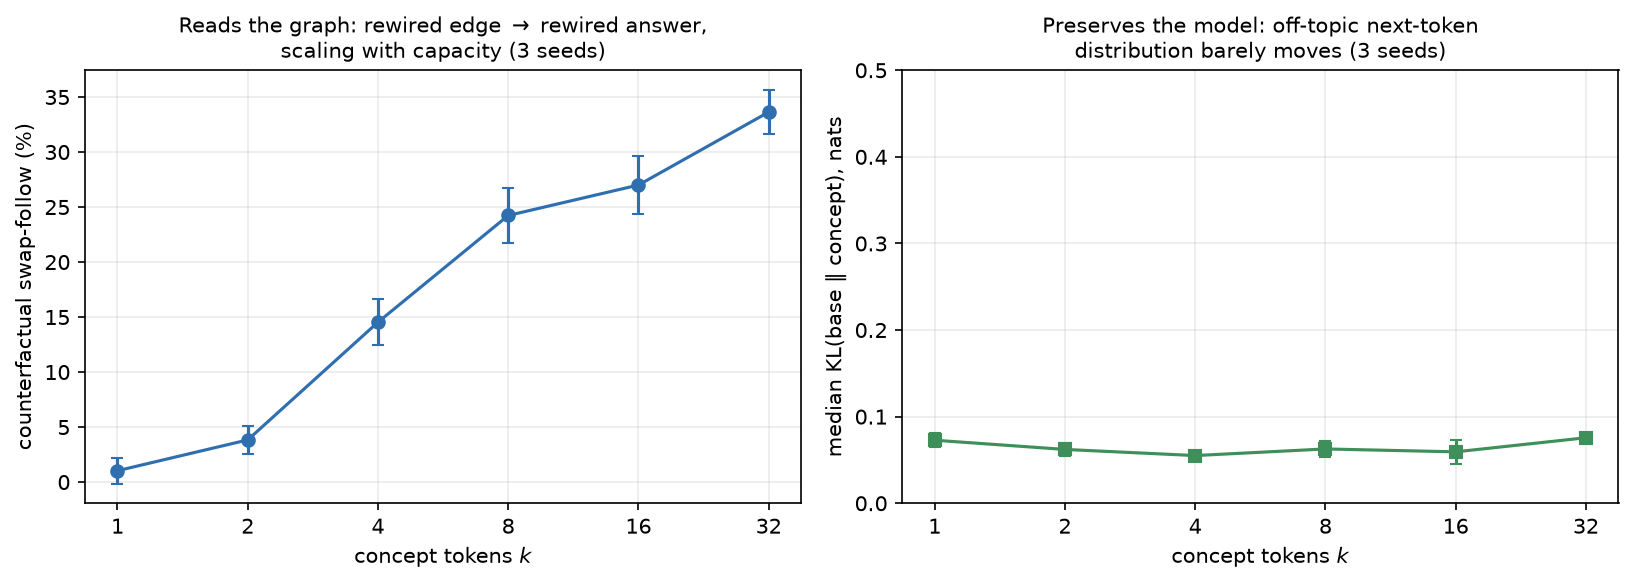
\includegraphics[width=\linewidth]{figures/fig_probes.png}
  \caption{Causal probes across $k$ (Qwen3-0.6B, 100k corpus, 400 single-fact probes per
  checkpoint, 3 seeds). Left: after rewiring the questioned edge to a type-plausible false
  neighbor, the model increasingly follows the graph to the \emph{false} answer --- the
  graph-reading signature, absent any parametric shortcut (the frozen base knows only 10\% of
  these probes). Right: on control tasks that mention the entity without asking about its
  facts, the next-token distribution barely moves, flat in $k$.}
  \label{fig:probes}
\end{figure}

A compression system can score well on QA while treating the graph as an opaque text-like
signal. Following the deficiency diagnosed across graph-token systems \citep{gteval,sink}, we
evaluate causally, by intervening on the \emph{input graph} of a trained model and re-encoding:
(a)~\emph{edge ablation} --- removing the questioned edge collapses accuracy on that question
(to 28--55\% depending on $k$) while removing an unrelated edge leaves it intact (90--96\%):
edges are encoded separably; (b)~\emph{counterfactual swap} --- rewiring the questioned edge to
a plausible false neighbor flips the model to the \emph{false} answer with probability rising
monotonically from $\sim$1\% at $k{=}1$ to $\sim$34\% at $k{=}32$
(Figure~\ref{fig:probes}, left; 3 seeds). Since the frozen base solves only 10\% of these
probes, parametric memory cannot explain the behavior: the concept tokens are causally
load-bearing, and faithfulness is \emph{capacity-limited rather than absent}. Meanwhile
injection does not disturb the model elsewhere: on off-topic control tasks the median
next-token KL between the model with and without concepts stays at 0.05--0.08 nats, flat in
$k$ (Figure~\ref{fig:probes}, right) --- by construction, since the student starts
bit-identical to the frozen model. Accuracy is also robust to prompt wording: across seven
system prompts (five seen styles, one held-out), \popqa{} accuracy of the $k{=}8$ model varies
with a standard deviation of $\le$1.1\,pt across 3 seeds.

\subsection{Ablations}

\begin{table}[t]
  \caption{Design ablations (10k corpus, $k{=}8$, 3 seeds each, strict held-out / full
  \popqa{}). Augmentation: pooled item-paired McNemar over 3 seeds; effect positive on average
  with seed-level heterogeneity (one seed reverses on \popqa{}).}
  \label{tab:ablations}
  \centering
  \small
  \begin{tabular}{llll}
    \toprule
    ablation & variants & held-out & note\\
    \midrule
    encoder capacity & 10M / 21M / \textbf{70M} / 231M & .423 / .441 / \textbf{.453} / .376 & peak at $\sim$70M; largest is worst\\
    placement & \textbf{prefix} / before / after / replace & \textbf{.453} / .423 / .434 / .380 & entity-adjacency does not help\\
    prompt augmentation & off / \textbf{on} & .453 / \textbf{.472} & \popqa{} $+2.0$\,pt; pooled $p{=}3{\times}10^{-36}$\\
    neighbor subsampling & \textbf{off} / on & $\Delta \approx 1$\,pt & null; cached teacher is $2\times$ faster\\
    \bottomrule
  \end{tabular}
\end{table}

Table~\ref{tab:ablations}: encoder capacity peaks near 70M parameters with the 231M encoder
clearly worst at this budget; placing concepts adjacent to (or in place of) the entity mention
does not beat a simple prefix; multi-prompt augmentation yields a small but, under pooled
paired testing, significant gain with real seed heterogeneity; per-step re-sampling of teacher
distractors is a null at our context budget.

\section{Discussion}

\paragraph{What governs the channel's value.} The results organize around a three-way trade.
Token budget buys accuracy monotonically but with diminishing returns; training data buys
unseen-entity generalization multiplicatively and had not saturated; and the two interact ---
tokens substitute for data. The model-size axis (Figure~\ref{fig:grid}) determines whether
these gains persist as the frozen model itself knows more; the two live interpretations --- a
\emph{ceiling effect} (bigger bases leave less headroom on the benchmark) versus a
\emph{steerability effect} (bigger frozen models need more training signal per unit of
behavioral change from $k$ soft tokens) --- make opposite predictions about whether more data
closes the gap, which the grid's 100k cells test directly. \todo{Finalize once 1.7B/4B cells
land.}

\paragraph{Limitations.} Single knowledge graph (Wikidata) and language (English);
entity-valued relations only (no literals); evaluation centered on \popqa{} and same-generator
held-out questions; faithfulness probes cover single-fact questions; corpora are
teacher-relative by design, so cross-backbone comparisons involve each model's own curriculum;
augmentation's effect is heterogeneous across seeds. Knowledge is injected for a single
identified entity mention per prompt; multi-entity composition is untested.

\paragraph{Outlook.} The encoder is modality-agnostic by construction --- its inputs are
embeddings, not text --- and extending concept tokens to multimodal knowledge (e.g., entity
images) for natively multimodal frozen models is the subject of ongoing work.

\section{Conclusion}

ConceptFormer-2 shows that a frozen, instruction-tuned language model can be grounded in a
knowledge graph through $k\!\approx\!8$ learned continuous tokens: $4.6\times$ over the frozen
base on unseen entities at one-tenth of retrieval's token cost, with causal evidence that the
graph is genuinely read and the model otherwise undisturbed. The value of the channel has
measurable structure --- monotone in tokens, multiplicative in data, interacting between the
two --- and the released corpora, checkpoints, and per-item evaluations make every number in
this paper re-derivable and extensible.

\begin{ack}
Drafted with substantial tooling assistance from Claude (Anthropic) for literature search,
evaluation-harness engineering, and manuscript preparation; all experimental design decisions,
runs, and claims were reviewed by the authors. \todo{Funding statements.}
\end{ack}

\small
\begin{thebibliography}{40}

\bibitem{cfv1} J.~Barmettler, A.~Bernstein, and L.~Rossetto.
\newblock ConceptFormer: Towards graph-native grounding of large language models via latent
  concept injection.
\newblock In \emph{Companion Proceedings of the ACM Web Conference 2026 (WWW Companion '26)},
  pp.~587--596, 2026. Best paper award, hosting workshop.
  \url{https://doi.org/10.1145/3774905.3794653}. arXiv:2504.07624.

\bibitem{xrag} X.~Cheng, X.~Wang, X.~Zhang, T.~Ge, S.~Chen, F.~Wei, H.~Zhang, and D.~Zhao.
\newblock xRAG: Extreme context compression for retrieval-augmented generation with one token.
\newblock NeurIPS 2024; arXiv:2405.13792.

\bibitem{icae} T.~Ge, J.~Hu, L.~Wang, X.~Wang, S.-Q.~Chen, and F.~Wei.
\newblock In-context autoencoder for context compression in a large language model.
\newblock ICLR 2024; arXiv:2307.06945.

\bibitem{gist} J.~Mu, X.~L.~Li, and N.~Goodman.
\newblock Learning to compress prompts with gist tokens.
\newblock NeurIPS 2023; arXiv:2304.08467.

\bibitem{autocompressor} A.~Chevalier, A.~Wettig, A.~Ajith, and D.~Chen.
\newblock Adapting language models to compress contexts.
\newblock EMNLP 2023; arXiv:2305.14788.

\bibitem{fivehundredx} Z.~Li, Y.~Su, and N.~Collier.
\newblock 500xCompressor: Generalized prompt compression for large language models.
\newblock arXiv:2408.03094, 2024.

\bibitem{pisco} M.~Louis, G.~Sidiropoulos, E.~Kanoulas, and V.~Nikoulina.
\newblock PISCO: Pretty simple compression for retrieval-augmented generation.
\newblock arXiv:2501.16075, 2025.

\bibitem{compllm} G.~Berton et al.
\newblock CompLLM: Compression for long context Q\&A.
\newblock arXiv:2509.19228, 2025.

\bibitem{arcencoder} H.~Dez\'{e}que et al.
\newblock ARC-Encoder: Learning compressed text representations for large language models.
\newblock arXiv:2510.20535, 2025.

\bibitem{cartridges} S.~Eyuboglu et al.
\newblock Cartridges: Lightweight and general-purpose long context representations via
  self-study.
\newblock arXiv:2506.06266, 2025.

\bibitem{overflow} Anonymous.
\newblock Detecting overflow in compressed token representations for retrieval-augmented
  generation.
\newblock arXiv:2602.12235, 2026.

\bibitem{kblam} X.~Wang, T.~Isazawa, L.~Mikaelyan, and J.~Hensman.
\newblock KBLaM: Knowledge base augmented language model.
\newblock ICLR 2025; arXiv:2410.10450.

\bibitem{knowledgeprompts} C.~N.~dos Santos, Z.~Dong, D.~Cer, J.~Nham, S.~Shakeri, J.~Ni, and
  Y.-H.~Sung.
\newblock Knowledge prompts: Injecting world knowledge into language models through soft
  prompts.
\newblock arXiv:2210.04726, 2022.

\bibitem{gnp} Y.~Tian, H.~Song, Z.~Wang, H.~Wang, Z.~Hu, F.~Wang, N.~V.~Chawla, and P.~Xu.
\newblock Graph neural prompting with large language models.
\newblock AAAI 2024; arXiv:2309.15427.

\bibitem{graphtoken} B.~Perozzi, B.~Fatemi, D.~Zelle, A.~Tsitsulin, M.~Kazemi, R.~Al-Rfou, and
  J.~Halcrow.
\newblock Let your graph do the talking: Encoding structured data for LLMs.
\newblock arXiv:2402.05862, 2024.

\bibitem{gretriever} X.~He, Y.~Tian, Y.~Sun, N.~V.~Chawla, T.~Laurent, Y.~LeCun, X.~Bresson,
  and B.~Hooi.
\newblock G-Retriever: Retrieval-augmented generation for textual graph understanding and
  question answering.
\newblock NeurIPS 2024; arXiv:2402.07630.

\bibitem{llaga} R.~Chen, T.~Zhao, A.~Jaiswal, N.~Shah, and Z.~Wang.
\newblock LLaGA: Large language and graph assistant.
\newblock ICML 2024; arXiv:2402.08170.

\bibitem{gteval} Anonymous.
\newblock Revisiting graph-tokenizing LLMs: A systematic evaluation.
\newblock arXiv:2605.03514, 2026.

\bibitem{sink} Anonymous.
\newblock When graph tokens sink: A mechanistic analysis of graph-token utilization in LLMs.
\newblock arXiv:2606.03712, 2026.

\bibitem{emptyshelves} Anonymous.
\newblock Empty shelves or lost keys? Disentangling encoding from recall of long-tail facts in
  language models.
\newblock arXiv:2602.14080, 2026.

\bibitem{headtotail} K.~Sun, Y.~E.~Xu, H.~Zha, Y.~Liu, and X.~L.~Dong.
\newblock Head-to-tail: How knowledgeable are large language models?
\newblock arXiv:2308.10168, 2023.

\bibitem{rag} P.~Lewis, E.~Perez, A.~Piktus, F.~Petroni, V.~Karpukhin, N.~Goyal,
  H.~K\"{u}ttler, M.~Lewis, W.-t.~Yih, T.~Rockt\"{a}schel, S.~Riedel, and D.~Kiela.
\newblock Retrieval-augmented generation for knowledge-intensive NLP tasks.
\newblock NeurIPS 2020.

\bibitem{lama} F.~Petroni, T.~Rockt\"{a}schel, S.~Riedel, P.~Lewis, A.~Bakhtin, Y.~Wu, and
  A.~Miller.
\newblock Language models as knowledge bases?
\newblock EMNLP 2019.

\bibitem{roberts} A.~Roberts, C.~Raffel, and N.~Shazeer.
\newblock How much knowledge can you pack into the parameters of a language model?
\newblock EMNLP 2020.

\bibitem{knowbert} M.~E.~Peters, M.~Neumann, R.~L.~Logan~IV, R.~Schwartz, V.~Joshi, S.~Singh,
  and N.~A.~Smith.
\newblock Knowledge enhanced contextual word representations.
\newblock EMNLP 2019.

\bibitem{kbert} W.~Liu, P.~Zhou, Z.~Zhao, Z.~Wang, Q.~Ju, H.~Deng, and P.~Wang.
\newblock K-BERT: Enabling language representation with knowledge graph.
\newblock AAAI 2020.

\bibitem{kadapter} R.~Wang, D.~Tang, N.~Duan, Z.~Wei, X.~Huang, J.~Ji, G.~Cao, D.~Jiang, and
  M.~Zhou.
\newblock K-Adapter: Infusing knowledge into pre-trained models with adapters.
\newblock Findings of ACL 2021.

\bibitem{transe} A.~Bordes, N.~Usunier, A.~Garc\'{i}a-Dur\'{a}n, J.~Weston, and O.~Yakhnenko.
\newblock Translating embeddings for modeling multi-relational data.
\newblock NeurIPS 2013.

\bibitem{pbg} A.~Lerer, L.~Wu, J.~Shen, T.~Lacroix, L.~Wehrstedt, A.~Bose, and
  A.~Peysakhovich.
\newblock PyTorch-BigGraph: A large scale graph embedding system.
\newblock MLSys 2019.

\bibitem{prefixtuning} X.~L.~Li and P.~Liang.
\newblock Prefix-tuning: Optimizing continuous prompts for generation.
\newblock ACL 2021.

\bibitem{lester} B.~Lester, R.~Al-Rfou, and N.~Constant.
\newblock The power of scale for parameter-efficient prompt tuning.
\newblock EMNLP 2021.

\bibitem{qineisner} G.~Qin and J.~Eisner.
\newblock Learning how to ask: Querying LMs with mixtures of soft prompts.
\newblock NAACL 2021.

\bibitem{textualinversion} R.~Gal, Y.~Alaluf, Y.~Atzmon, O.~Patashnik, A.~H.~Bermano,
  G.~Chechik, and D.~Cohen-Or.
\newblock An image is worth one word: Personalizing text-to-image generation using textual
  inversion.
\newblock ICLR 2023.

\bibitem{frozenlm} M.~Tsimpoukelli, J.~Menick, S.~Cabi, S.~M.~A.~Eslami, O.~Vinyals, and
  F.~Hill.
\newblock Multimodal few-shot learning with frozen language models.
\newblock NeurIPS 2021.

\bibitem{perceiver} A.~Jaegle, F.~Gimeno, A.~Brock, A.~Zisserman, O.~Vinyals, and J.~Carreira.
\newblock Perceiver: General perception with iterative attention.
\newblock ICML 2021.

\bibitem{flamingo} J.-B.~Alayrac et al.
\newblock Flamingo: A visual language model for few-shot learning.
\newblock NeurIPS 2022.

\bibitem{wikidata} D.~Vrande\v{c}i\'{c} and M.~Kr\"{o}tzsch.
\newblock Wikidata: A free collaborative knowledgebase.
\newblock Communications of the ACM, 57(10):78--85, 2014.

\bibitem{talklikeagraph} B.~Fatemi, J.~Halcrow, and B.~Perozzi.
\newblock Talk like a graph: Encoding graphs for large language models.
\newblock ICLR 2024; arXiv:2310.04560.

\bibitem{popqa} A.~Mallen, A.~Asai, V.~Zhong, R.~Das, D.~Khashabi, and H.~Hajishirzi.
\newblock When not to trust language models: Investigating effectiveness of parametric and
  non-parametric memories.
\newblock ACL 2023; arXiv:2212.10511.

\bibitem{hinton} G.~Hinton, O.~Vinyals, and J.~Dean.
\newblock Distilling the knowledge in a neural network.
\newblock arXiv:1503.02531, 2015.

\bibitem{qwen} Qwen Team.
\newblock Qwen3 model family.
\newblock Technical reports, 2025; \url{https://huggingface.co/Qwen}.

\end{thebibliography}

\end{document}
